\section{A bit of Quantum Physics}

\begin{frame}{The Schrödinger equation}

Quantum Physics describes phenomenons at the scale of atoms and particles\newline


The Schrödinger equation is primarily important
\begin{equation*}
        i\hbar\frac{\partial}{\partial t}\Psi(x,t)=-\frac{\hbar^2}{2m}\nabla^2\Psi(x,t)+V(x,t)\Psi(x,t).
\end{equation*} 
On note que
\begin{itemize}
    \item it takes its value in $\mathbb{C}$, we can notice the $i$ from pure imaginary number on the left handside. 
    \item we notice the $\nabla$ operator from differential geometry, it's used in Maxwell equations
    (electromagnetism) and in Navier-Stokes equation (hydrodynamic)
    \item $\hbar = \frac{h}{2\pi}$ where $h$ is the Planck's constant ($h = 6,62607015.10^{-34} J.s$) 
    \item actions on quantum objects are unitary operators within an Hilber vector space.
\end{itemize}
\end{frame}

\begin{frame}{Consequence of the Schrödinger equation}
Several things result from te Schrödinger equation 
\begin{itemize}
    \item quantum phenomenons take discrete value or \textit{quantas}
    \item quantum objects do not continuously go from one state to another
    \item quantum objects can exist in a superposition of several states at the same time.
    \item quantum objects can simultaneously waves and particles
\end{itemize}
\begin{center}
    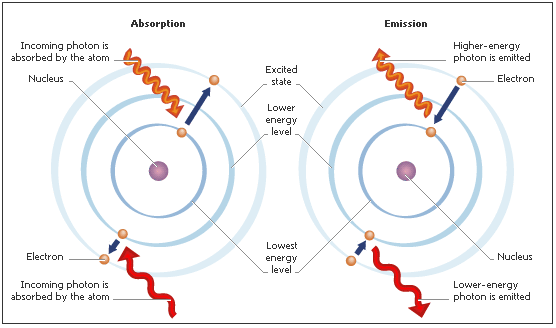
\includegraphics[width=0.50\textwidth]{images/photon.png}    
\end{center}
\end{frame}

\begin{frame}{Superposition}
Quantum objects are linear combinations of basic states, belonging to an orthonormal basis, such as
\begin{equation*}
    \ket{\Psi} = \alpha\ket{0}+\beta\ket{1}+\gamma\ket{2}+\delta\ket{3}
\end{equation*}
Complex coefficients $\alpha$, $\beta$, $\gamma$ et $\delta$ are \textit{complex probabilities}
\begin{itemize}
    \item they respect the normalisation rule$|\alpha|^2+|\beta|^2+|\gamma|^2+|\delta|^2 = 1$
    \item each square of the coefficient module shows the probability to measure the related state (we have a  
    probability $|\alpha|^2$ to see state$\ket{0}$ when observing $\ket{\psi}$
\end{itemize}
\end{frame}

\begin{frame}{Observation and quantum collapse}
In Quantum Physics, observation is a destruction operation, it alters the watched state
\begin{equation*}
    \ket{\Psi} = \alpha\ket{0}+\beta\ket{1}+\gamma\ket{2}+\delta\ket{3}
\end{equation*}
Observing $\ket{\Psi}$ will result in\textbf{collapsing} state $\ket{\Psi}$ on one of the 4~possible states
\begin{itemize}
    \item we see only one of those states, not the 3 other ones
    \item once $\ket{\Psi}$ is collapsed, it won't change anymore. 
\end{itemize}
With Quantum Computing, we build an "intrumented quentum physics experience", we can repeat the experience that builds
 $\ket{\Psi}$ as many times as required
\begin{itemize}
    \item by doing several "shots", we know the probability of each "base state"
    \item \textbf{BEWARE~:} we know the squares of the coefficients's modules (as complex numbers) not the value themselves
    (we mesure $|\alpha|^2$ and not $\alpha$) 
    \item we have no access to the whole information ccarried by  $\ket{\Psi}$
    \item particularily, "phase factors" (written as $e^{i\theta}$) are invisible because they are unitary. 
\end{itemize}
\end{frame}

\begin{frame}{Entanglement}
Entanglement is a very anti-intuitive concept\newline

Einstein did not believed in it, he wrote the famoux EPR (Einstein-Podolsky-Rosen) in 1934\newline

In 1982, the experience by Alain Aspect prooved that entanglement was real, we won the Nobel Price in 2022. \newline

An entangled state groups several particles that should be considered as a single quantum object
\begin{itemize}
    \item when two particles $A$ et $B$ are entangled, whatever acts on $A$ acts on  $B$ too, it actually operates on 
    the entangled system $A \otimes B$
    \item we can't separate $A$ and $B$, they should be handled together
    \item entanglement is no interactation, it is not impacted by distance
    \item in particular, measuring $A$collapses it and collapses $B$ too, simultaneously. 
\end{itemize}
\end{frame}

\begin{frame}{Basements of quantum computing}
Quantum Computing is based on the 3 principles of quantum physics
\begin{itemize}
    \item superposition helps in encoding information in quantum states within several \textit{qubits}
    \item entanglement helps building complex systems made of several qubits
    \item Interference makes it possible to build unitary operation as well as mesure operators. Mesuring always results
    in collapsing the states
\end{itemize}
\end{frame}

\begin{frame}{Concrete mathematical basements}
Quantum physics can be implemented via very concrete mathematics
La physique quantique s'appuie sur un socle mathématique très solide~:
\begin{itemize}
    \item  quabits exist within a 2 dimension $\mathbb{C}$-fied, it is an Hilbert field
    \itemà $n$ qubits systems exist in a Hilbeet field whose dimension is $2^n$
\end{itemize}
Mathematically we can describe
\begin{itemize}
    \item the operators acting on quabits (vectors in a field)
    \item how qubits interact tohether
    \item qubit measurement
    \item formal expression of entanglement
\end{itemize}
Quantum Physics often makes use lots of linear algebra in Hibert fields.
\end{frame}

\begin{frame}{Main ideas expressed here}
Fundamentally, quantum programming is
\begin{itemize}
    \item an intrumented experience of Quantum Physics
    \item smart use of a quantum mechanics phenomenons to accelerate some HPC steps 
    \begin{itemize}
        \item these steps, mapped on QC expeirences, are of complexity NP-C, QC make NP problems reachable by HPC
        \item HPC will always be required to bootstrap QC 
    \end{itemize}
\end{itemize}
Most of the time, QC is good to identift the charactéeristics of a known gloabl property 
\begin{itemize}
    \item given a function $f$,  periodic, what is its period ? (Shor)
    \item given a function $f$  null almost everywhere what are the $x$ such as $f(x) \neq 0$ ? (Grover)
    \item identifying  minima and maxima of quadratic function expressed as matrices (QUBO)
    \item identifying the properties of a graph (MIS, MVC, Clique, MaxCut,...) 
\end{itemize}
\end{frame}


